\section{M\"obius Groups}

\begin{definition}[M\"obius transformation]
A M\"obius transformation (or map) is a function of a complex variable $z$ that can be written in the form 
\begin{align*}
    f(z) = \frac{az + b}{cz + d}
\end{align*} for some $a, b, c, d \in \mathbb{C}$ with $ad - bc \neq 0$.
\end{definition} 

Why $ad - bc \neq 0$?
\begin{align*}
    f(z) - f(w) &= \frac{(ad - bc)(z - w)}{(cz + d) (cw + d)}.
\end{align*} 
So, $ad - bc = 0 \implies f$ is constant (not interesting).
If,  $ad - bc \neq 0 \implies f$ is injective.

When does $f(z) = g(z)$ ($g(z)$ is $f(z)$ with different $a, b, c, d$)?
Suppose $\exists$ at least 3 values of $z$ in $\mathbb{C}$ s.t. 
\begin{align*}
    \frac{az + b}{cz + d} &= \frac{\alpha z + \beta}{\gamma z + \delta} \\
    ad - bc &\neq 0 \alpha \delta - \beta \gamma \neq 0.
\end{align*}
Then $\exists \; \lambda \neq 0, \lambda \in \mathbb{C}$ s.t. 
\begin{align*}
    \begin{pmatrix}\alpha & \beta \\\gamma & \delta\end{pmatrix} &= \lambda \begin{pmatrix}a & b \\c & d\end{pmatrix}. 
\end{align*} 
Since, we have 3 distinct values of $z$ for which 
\begin{align*}
    (az + b)(\gamma z + \delta)&= (\alpha z + \beta)(cz + d)
    \intertext{so these quadratics are identical}
    \implies \alpha \gamma &= \alpha c,\ b \delta = \beta d \\
    a \delta + \beta \delta &= \alpha d + \beta c \\
    \text{Let } \mu &= a \delta - \beta c = \alpha d - b \gamma \\
    (\text{so } \mu^2 &= (ad - bc)(\alpha \delta - \beta \gamma) \neq 0). \\
    \text{Then } \begin{pmatrix}d & -b \\-c & a\end{pmatrix} \begin{pmatrix}\alpha & \beta \\\gamma & \delta\end{pmatrix} &= \begin{pmatrix}\mu & 0 \\0 & \mu\end{pmatrix} \\
    \implies \begin{pmatrix}\alpha & \beta \\\gamma & \delta\end{pmatrix} &= \frac{\mu}{ad - bc} \begin{pmatrix}a & b \\c & d\end{pmatrix}.
\end{align*} 

Problem: $f$ is not defined at $z = - \frac{d}{c}$.
We would like $f(-\frac{d}{c}) = \infty$.
We consider $f$ defined on $\mathbb{C} \cup \{ \infty \} = \mathbb{C}_\infty$ the extended complex plane.
So if $f(z) = \frac{az + b}{cz + d}$, domain is now $\mathbb{C}_\infty$.
If $c \neq 0;\ f(\infty) = \frac{a}{c};\ f(-\frac{d}{c}) = \infty$ else $c = 0;\ f(\infty) = \infty$.

\begin{figure}
    \centering
    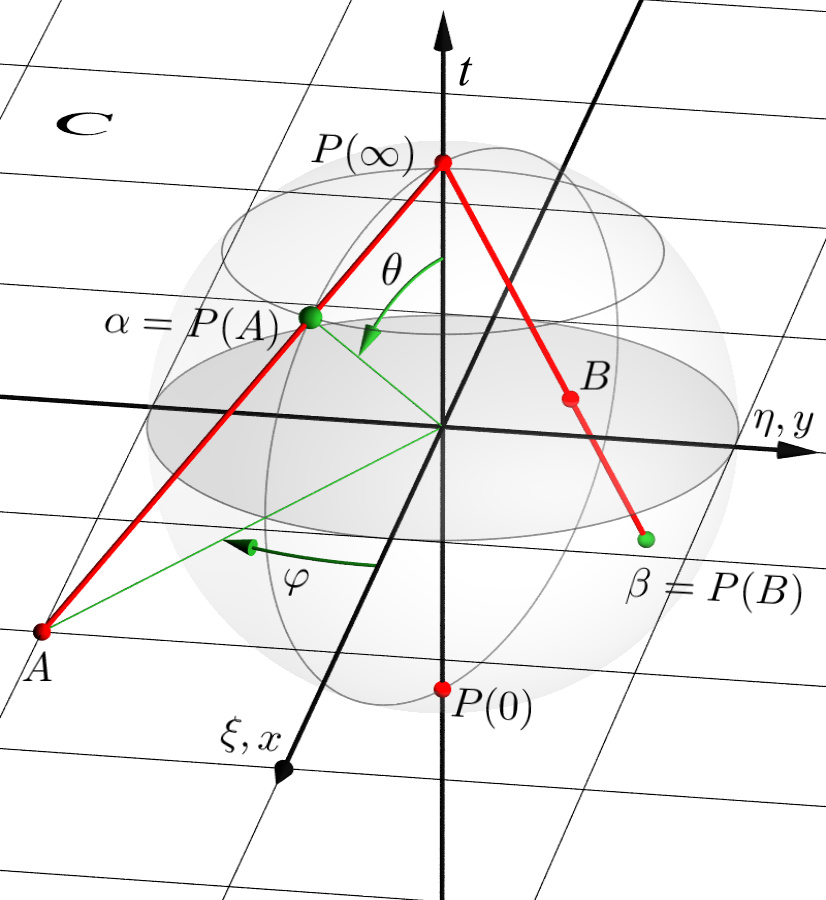
\includegraphics[height=5cm]{07-RiemannSphere.png}
    \caption{Stereographic projection of a complex number $A$ onto a point $\alpha$ of the Riemann sphere}
\end{figure} 

\begin{theorem}\label{thm:14}
    The set $\mathcal{M}$ of all M\"obius maps on $\mathbb{C}_\infty$ is a group under composition.
    It is a subgroup of $\operatorname{Sym}(\mathbb{C}_\infty)$.
\end{theorem} 

\begin{proof}
    \begin{itemize}
        \item Composition of maps is associative.
        \item $I(z) = z \in \mathcal{M}$ ($a = d = 1, c = d = 0$)
        \item closure:
        \begin{align*}
            \text{Let } f(z) &= \frac{az + b}{cz + d},\ g(z) = \frac{\alpha z + \beta}{\gamma z + \delta} \\
            \text{Suppose } c &\neq 0,\ \delta \neq 0 \\
            \text{First suppose } z &\in \mathbb{C} \setminus \{ - \delta / \gamma \} \\
            \text{Then } f(g(z)) &=  \frac{a \left( \frac{\alpha z + \beta}{\gamma z + \delta} \right) + b}{c \left( \frac{\alpha z + \beta}{\gamma z + \delta} \right) + d} \\
            &= \frac{(a \alpha + b \gamma) z + (a \beta + b \delta)}{(c \alpha + d \gamma)z + (c \beta + \delta d)} \\
            &\in \mathcal{M} \\
            \text{since} (a \alpha + b \gamma)(c \beta + \delta d) - (a \beta + b \delta)(c \alpha + d \gamma) &= (ad - bc)(\alpha \delta - \beta \gamma) \neq 0 \\
            \text{Also, } f\left(g\left(-\frac{\delta}{\gamma}\right)\right) &= f(\infty) = \frac{a}{c} \\
            \text{and } \frac{(a \alpha + b \gamma) \left(-\frac{\delta}{\gamma}\right) + (a \beta + b \delta)}{(c \alpha + d \gamma)\left(-\frac{\delta}{\gamma}\right) + (c \beta + \delta d)} &= \frac{a \alpha \left(-\frac{\delta}{\gamma}\right) + \alpha \beta}{c \alpha \left(-\frac{\delta}{\gamma}\right) + c \beta} \\
            &= \frac{a}{c} \checkmark \\
            \text{Need to check } c &= 0
        \end{align*} 
        \item Inverses: 
        \begin{align*}
            f(z) &= \frac{az + b}{cz + d},\ ad - bc \neq 0 \\
            \text{Let } f^*(z) &= \frac{dz - b}{-cz + a} \\
            \text{Then } f(f^*(z)) &= z = f^*(f(z)) \text{ for } z \neq -\frac{d}{c}, -\frac{a}{c}, \infty 
            \intertext{These cases are ok.}
            \text{If } c &= 0 \\
            f(f^*(\infty)) &= f(\infty) = \infty = f^*(f(\infty)).
        \end{align*}
    \end{itemize} 
\end{proof} 

\begin{theorem}\label{thm:15}
    $\operatorname{GL}_2(\mathbb{C}) / Z \cong \mathcal{M}$ where $Z = \left\{ \begin{pmatrix}\lambda & 0 \\0 & \lambda\end{pmatrix} : \lambda \in \mathbb{C} \setminus \{0\} \right\}$ ($Z$ is the centre of $\operatorname{GL}_2(\mathbb{C})$).
\end{theorem} 

\begin{proof}
    We construct a surjective homomorphism from $\operatorname{GL}_2(\mathbb{C})$ onto $\mathcal{M}$ with kernel $Z$.
    \begin{align*}
        \text{Let } \Phi : \operatorname{GL}_2(\mathbb{C}) &\to \mathcal{M} \\
        \begin{pmatrix}a & b \\c & d\end{pmatrix} &\mapsto f(z) = \frac{az + b}{cz + d}
        \intertext{Note $\Phi$ is a homomorphism}
        f(z) &= \frac{az + b}{cz + d},\ g(z) = \frac{\alpha z + \beta}{\gamma z + \delta} \\
        \Phi \left( \begin{pmatrix}a & b \\c & d\end{pmatrix} \right) &\Phi \left( \begin{pmatrix}\alpha & \beta \\\gamma & \delta\end{pmatrix} \right) (z) = f \circ g(z) \\
        &= \frac{(a \alpha + b \gamma) z + (a \beta + b \delta)}{(c \alpha + d \gamma)z + (c \beta + \delta d)} \text{ from proof of \Cref{thm:14}} \\
        &= \Phi \left( \begin{pmatrix}a & b \\c & d\end{pmatrix} \begin{pmatrix}\alpha & \beta \\\gamma & \delta\end{pmatrix} \right) (z).
    \end{align*} 
    Clearly $\Phi$ is surjective.
    \begin{align*}
        \begin{pmatrix}a & b \\c & d\end{pmatrix} &\in \ker \Phi \\
        \iff \frac{az + b}{cz + d} &= z \; \forall \; z \in C_\infty \\
        \text{Let } z &= 0 \implies c = 0 \\
        z &= 0 \implies b = 0 \\
        z &= 1 \implies a = d \\
        \implies \ker \Phi &= Z
    \end{align*} 
    Finally apply \nameref{thm:six}.
\end{proof} 